\section{Hardware support}

The embedded world is responsible for the majority of the world's microcontrollers.
The diversity of CPU keep increasing every year.
Working with this diversity of constrained devices makes the developer's work harder as he needs to adapt and learn to use specific libraries for each device.
A source code on a particular device will not be easily reusable for another device.

With RTOS, developers can more easily make their code portable on many devices.

This section first describes the three classes of constrained devices and how this is related to RTOS.
Then, it explains what a hardware abstraction layer (HAL) is and how RTOS uses it in order to be compatible with the largest number of devices.

\subsection{Constrained device classes}

Constrained devices have been classified into 3 classes by the Internet Engineering Task Force (IETF) with the request for comments RFC7228\cite{RFC7228} in May 2014.
IETF is a standards organization aiming at improving and maintaining the usability of the Internet.
Therefore they play a certain role in the evolution of IoT technologies.
We can argue that IETF is a competent authority over constrained devices since its domain of competence is the Internet.
Nonetheless, the boundary between constrained embedded devices and the Internet is permeable.
For the purpose of this thesis, the classification they made with RFC7228 is used.
RFCs are informational or experimental documents published by engineers and computer scientists.
Some of them become standards and some others are \textit{de facto} standards.

The distinction between the three classes are made with the random-access memory (RAM) and read-only memory (ROM) capabilities of each device.
Table \ref{tab:constrained-devices-classes} resumes the different constrained device classes.

\begin{table}[!h]
  \centering
  \begin{tabular}{|l|l|l|}
  \hline
   & Data size (e.g., RAM) & Code size (e.g., flash) \\ \hline
  Class 0 (C0) & \textless{}\textless{} 10 kB & \textless{}\textless{} 100 kB \\ %\hline
  Class 1 (C1) & $\sim$ 10 kB & $\sim$ 100 kB \\ %\hline
  Class 2 (C2) & $\sim$ 50 kB & $\sim$ 250 kB \\ \hline
  \end{tabular}
  \caption{classes of constrained devices}
  \label{tab:constrained-devices-classes}
\end{table}

\paragraph{Class 0.}
These devices are the most constrained.
They are typically sensor nodes (or motes) in a sensor network.
There are so constrained that they cannot access the Internet without the help of a larger device.
The source code of a RTOS is often too heavy to fit in such devices.
Instead Class-0 devices are usually used bare metal.
In the embedded world, bare-metal programming is writing code that runs directly on the hardware without any abstraction such as an OS.

\paragraph{Class 1.}
These devices are able to talk to each other but via constrained protocols.
The use of security protocols are often too heavy for that class.
%RTOS mainly target this kind of devices.
RTOS generally require at least a few kB for the strict minimal functionalities to run.
Therefore, they are not practical for class 0 devices (even if they could technically run) and mainly target class 1 or more powerful devices.


\paragraph{Class 2.}
These devices are the less constrained and can use the same stacks of protocols used in personal computers and servers.
General-purpose OS can be used for this kind of device but the class-2 devices can benefit from lightweight and energy-efficient protocols.

\subsection{Hardware abstraction layer}

Due to the variety of CPU, vendors provide a set of libraries used to develop applications on their architectures.
This set of libraries and tools are called the hardware abstraction layer.

\paragraph{Definition of HAL}
% TODO
% Repetition of 'hardware'
A hardware abstraction layer defines a set of routines, protocols and tools to access underlying hardware.
It provides abstract and high-level functions to interact with the hardware.
The hardware, drivers and board supports are considered as black boxes.

\paragraph{RTOS and HAL}
The HAL is strongly dependent on the architecture of the CPU.
In order for the RTOS to support multiple boards and architectures, it has to implement and use the different HAL provided by the vendors.

\begin{figure}[!h]
  \centering
  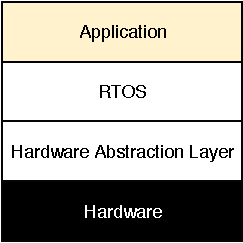
\includegraphics[scale=1]{assets/hal-layers.pdf}
  \caption{\label{fig:hal-layer}layers around the hardware abstraction layer}
\end{figure}

Figure \ref{fig:hal-layer} shows that the application and RTOS layers are placed above the HAL, itself just above the device layer.
The application layer talks to the RTOS and the RTOS layer talks to the corresponding HAL depending on the device used.

%TODO rework this part
\paragraph{Pro and cons}
Developers can switch hardware and perform cross-platform testing more easily.
But there is some limitation: the HAL is tied to the hardware and change heavily with it.
Also, there is some limitation using a hardware abstraction layer.
Not all the functionalities from the hardware are available.